\begin{refsection}[research/nakajima/group.bib]
\nocite{*}
\chapter{Computational Molecular Science Research Team}

\section{Members}

\begin{itemize}
  \item[] Takahito Nakajima (Team Leader)
  \item[] Tomomi Shimazaki (Senior Scientist)
  \item[] Noriyuki Minezawa (Senior Scientist)
  \item[] Michio Katouda (Research Scientist)
  \item[] Taichi Kosugi (Research Scientist)
  \item[] Tomoki Kobori (Research Scientist)
  \item[] Keisuke Sawada (Research Scientist)
  \item[] Muneaki Kamiya (Visiting Scientist)
  \item[] Yutaka Nakatsuka (Visiting Scientist)
\end{itemize}

\section{Research Activities}
\subsection{Development of original molecular theory}
An atomic- and molecular-level understanding of drug actions and the mechanisms of a variety of chemical reactions will provide insight for developing new drugs and materials.
Although a number of diverse experimental methods have been developed, it still remains difficult to investigate the state of complex molecules and to follow chemical reactions in detail.
Therefore, a theoretical molecular science that can predict the properties and functions of matter at the atomic and molecular levels by means of molecular theoretical calculations is keenly awaited as a replacement for experiment.
Theoretical molecular science has recently made great strides due to progress in molecular theory and computer development.
However, it is still unsatisfactory for practical applications.
Consequently, our main goal is to realize an updated theoretical molecular science by developing a molecular theory and calculation methods to handle large complex molecules with high precision under a variety of conditions.
To achieve our aim, we have so far developed several methods of calculation.
Examples include a way for resolving a significant problem facing conventional methods of calculation, in which the calculation volume increases dramatically when dealing with larger molecules;
a way for improving the precision of calculations in molecular simulations;
and a way for high-precision calculation of the properties of molecules containing heavy atoms such as metal atoms. 

\subsection{New molecular science software NTChem}
Quantum chemistry software comprises immensely useful tools in material and biological science research.
Widely diverse programs have been developed in Western countries as Japan has lagged.
In fact, only a few programs have been developed in Japan.
The mission of our research team is to provide K computer users with a high-performance software for quantum molecular simulation.
In the early stage of the K computer project, no quantum chemistry software was available for general purpose and massively parallel computation on the K computer because not every program was designed for use on it.
Therefore, we have chosen to develop a new comprehensive ab initio quantum chemistry software locally: NTChem.
NTChem is completely new software that implements not only standard quantum chemistry approaches, but also original and improved theoretical methods that we have developed in our research work.
The main features of the current version, NTChem2013, are the following:
\begin{enumerate}
\renewcommand{\labelenumi}{\arabic{enumi}).}
\setlength{\itemsep}{0cm}
\item Electronic structure calculation of the ground state of atoms and molecules based on Hartree–Fock (HF) and density functional theory (DFT) methods.
\item Linear-scaling or low-scaling DFT: Gaussian and finite-element Coulomb (GFC) resolution-of-the-identity (RI) DFT, pseudospectral DFT/HF, and dual-level DFT. 
\item Low-scaling SCF calculation using diagonalization-free approaches: purification density matrix, pseudo-diagonalization, and quadratic convergence SCF. 
\item Excited-state DFT calculation: time-dependent DFT (TDDFT) and transition potential (DFT-TP). 
\item Accurate electron correlation methods for ground and excited states: M{\o}ller–Plesset perturbation theory, coupled-cluster (CC) theory, and quantum Monte Carlo (QMC) method.
\item Massively parallel computing on the K computer and Intel-based architectures: HF, DFT, resolution-of-the-identity second-order M{\o}ller–Plesset (RI-MP2) method, and QMC method.
\item Two-component relativistic electronic structure calculation with spin–orbit interactions: Douglas–Kroll (DK) (DK1, DK2, and DK3), regular approximation (RA) (zeroth-order RA (ZORA) and infinite-order RA (IORA)), and Relativistic scheme for Eliminating Small Components (RESC).
\item Model calculations for large molecular systems: quantum mechanics/molecular mechanics (QM/MM) and Our own N-layered Integrated molecular Orbital and molecular Mechanics (ONIOM). 
\item Calculation of solvation effects: COnductor-like Screening MOdel (COSMO) (interfaced with the HONDO program), averaged solvent electrostatic potential/molecular dynamics (ASEP/MD), and QM/MM-MD.
\item Efficient calculation for chemical reaction pathway.
\item Ab initio molecular dynamics calculation.
\item Calculation of magnetic properties: nuclear magnetic resonance (NMR) chemical shifts, magnetizabilities, and electron paramagnetic resonance (EPR) g tensors.
\item Population analysis: Mulliken and natural bond orbital (NBO) analysis (interfaced with NBO 6.0).
\item Orbital interaction analysis: maximally interacting orbital (MIO) and paired interacting orbital (PIO) methods.
\end{enumerate}

\section{Research Results and Achievements}
\subsection{Development of original molecular theory and software}
\subsubsection{Fast estimations of two-electron repulsive integrals using Pseudospectral method}
A fast estimation of two-electron repulsive integrals (ERIs) is an important and imperative subject in any ab initio quantum chemical calculationsa.
Since the computational cost of the ERIs formally increases as $N^4$, where $N$ is the number of basis functions, we often suffer from much time-consuming estimations in large molecular systems.
In order to address the tough problem, several methodologies have been developed to date.
Among them, the pseudospectral (PS) method is a strong candidate for a quick and efficient evaluation of the ERIs.
In the PS method, one analytical integral is replaced by a numerical summation consisting of discrete grid points so that the computational cost is reduced from $O(N^4)$ to $O(MN^2)$, where $M$ is the number of grid points.
Because of the discretization of a continuous integral space, the PS method is not only fast in estimations of the ERIs but also suitable for recent massively parallel computations using numerous CPU cores.
Nevertheless, ab initio quantum chemical calculations with the PS method have never demonstrated in large molecular systems which contains more than 1,000 atoms.
To this end, we implement the PS and PS-GAP methods into our NTChem program and investigate the performances of these methods using the MPI-parallelized code.
The PS-GAP method is a further accelerated method that the PS and Gaussian and plane-wave (GAPW) methods are combined. 
In the following all quantum chemical calculations, the pure density functional theory was adopted, and the Kohn–Sham orbital was expanded by Def2-SVP Gaussian basis set.
We employed one-dimensionally polymerized glucose-alanine chain and three-dimensionally distributed H$_2$O molecular cluster as test systems.
The largest size system is constituted by 1,226 atoms and 10,128 basis functions.
The LIBINT library was utilized in computations of analytical integrals, and the parallel FFTW library was exploited in the GAPW and PS-GAP methods.
The performance check of PS and PS-GAP methods was conducted on the Research Center for Computational Science (RCCS) and the K computer system. First, we investigated computational scalings of the PS and PS-GAP methods with respect to the number of basis functions.
We performed MPI computations using 16 CPU cores on the RCCS and compare the computational times of the ERIs among usual analytical, GAPW, PS, and PS-GAP methods.
Figure~\localref{fig:ps_basis}  exhibits the computational times as a function of the number of basis functions.
We find that the PS-GAP method is much faster than the other methods whereas the PS method is the slowest among all methods.
Moreover, the PS-GAP method is found to achieve the low-dimensional scaling by less than square.
This suggests that the PS-GAP method allows us fast calculations even for much larger systems than present maximum size one.
Next, we examined parallel efficiencies of PS and PS-GAP methods in terms of large-scale parallel computations.
The glucose-alanine chain with 8,202 basis functions and H$_2$O molecular cluster with 10,128 basis functions were adopted for test systems.
We carried out MPI/OpenMP hybrid computations using eight threads per one MPI process.
One MPI process was assigned to one node on the K Computer.
Figure~\localref{fig:ps_node} shows the computational time of the ERIs as a function of used nodes.
As well as the test of computational scalings on the RCCS, we realize the fast evaluation of the ERIs using the PS-GAP method.
For the efficacy of large-scale parallelization, the PS method shows a good parallel efficiency whereas the PS-GAP method seems to quickly saturate with nodes.
On the other hand, we find that the conventional analytical method also shows a good efficiency and is faster than the PS method in the case of the H$_2$O molecular cluster.

\begin{figure}[b]
\centering
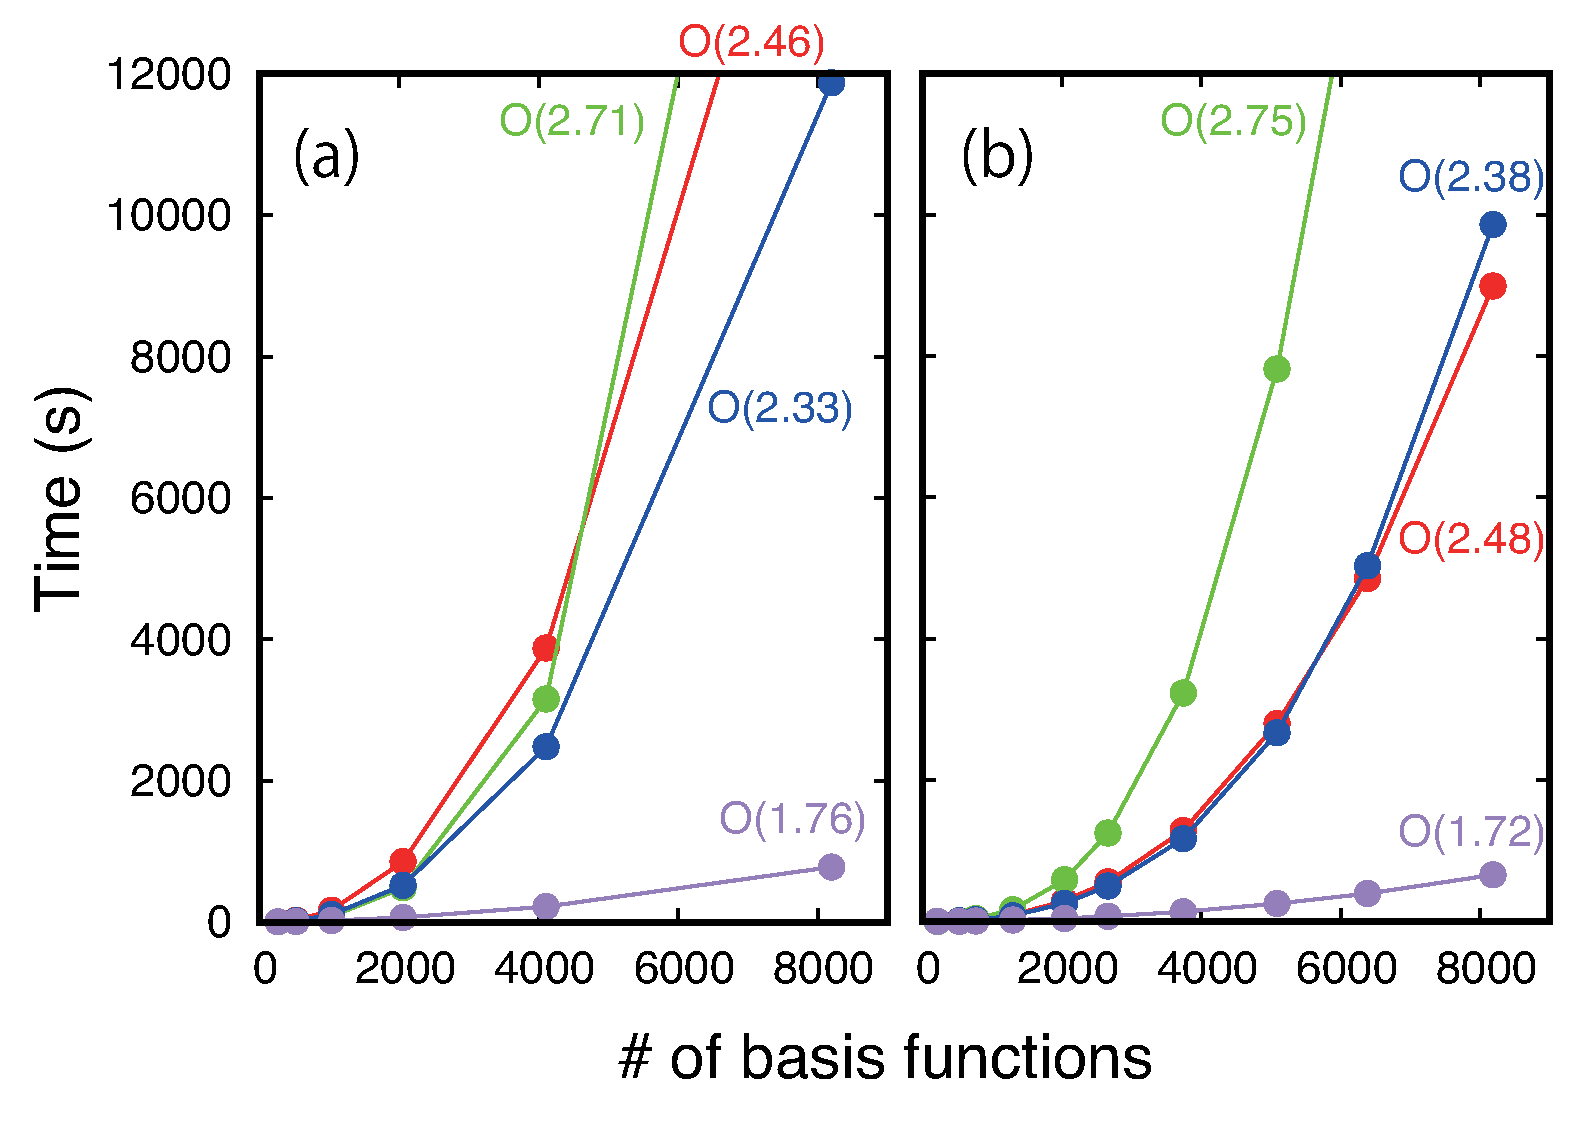
\includegraphics[width=0.525\textwidth]
{research/nakajima/ps_basis.eps}
\caption{Computational time of two-electron repulsive integrals in glucose-alanine chain (a) and H$_2$O molecular cluster (b) as a function of the number of basis functions.
The red, blue, green, and purple circles denote the analytical, GAPW, PS, and PS-GAP methods, respectively.}
\locallabel{fig:ps_basis}
\end{figure}

\begin{figure}[t]
\centering
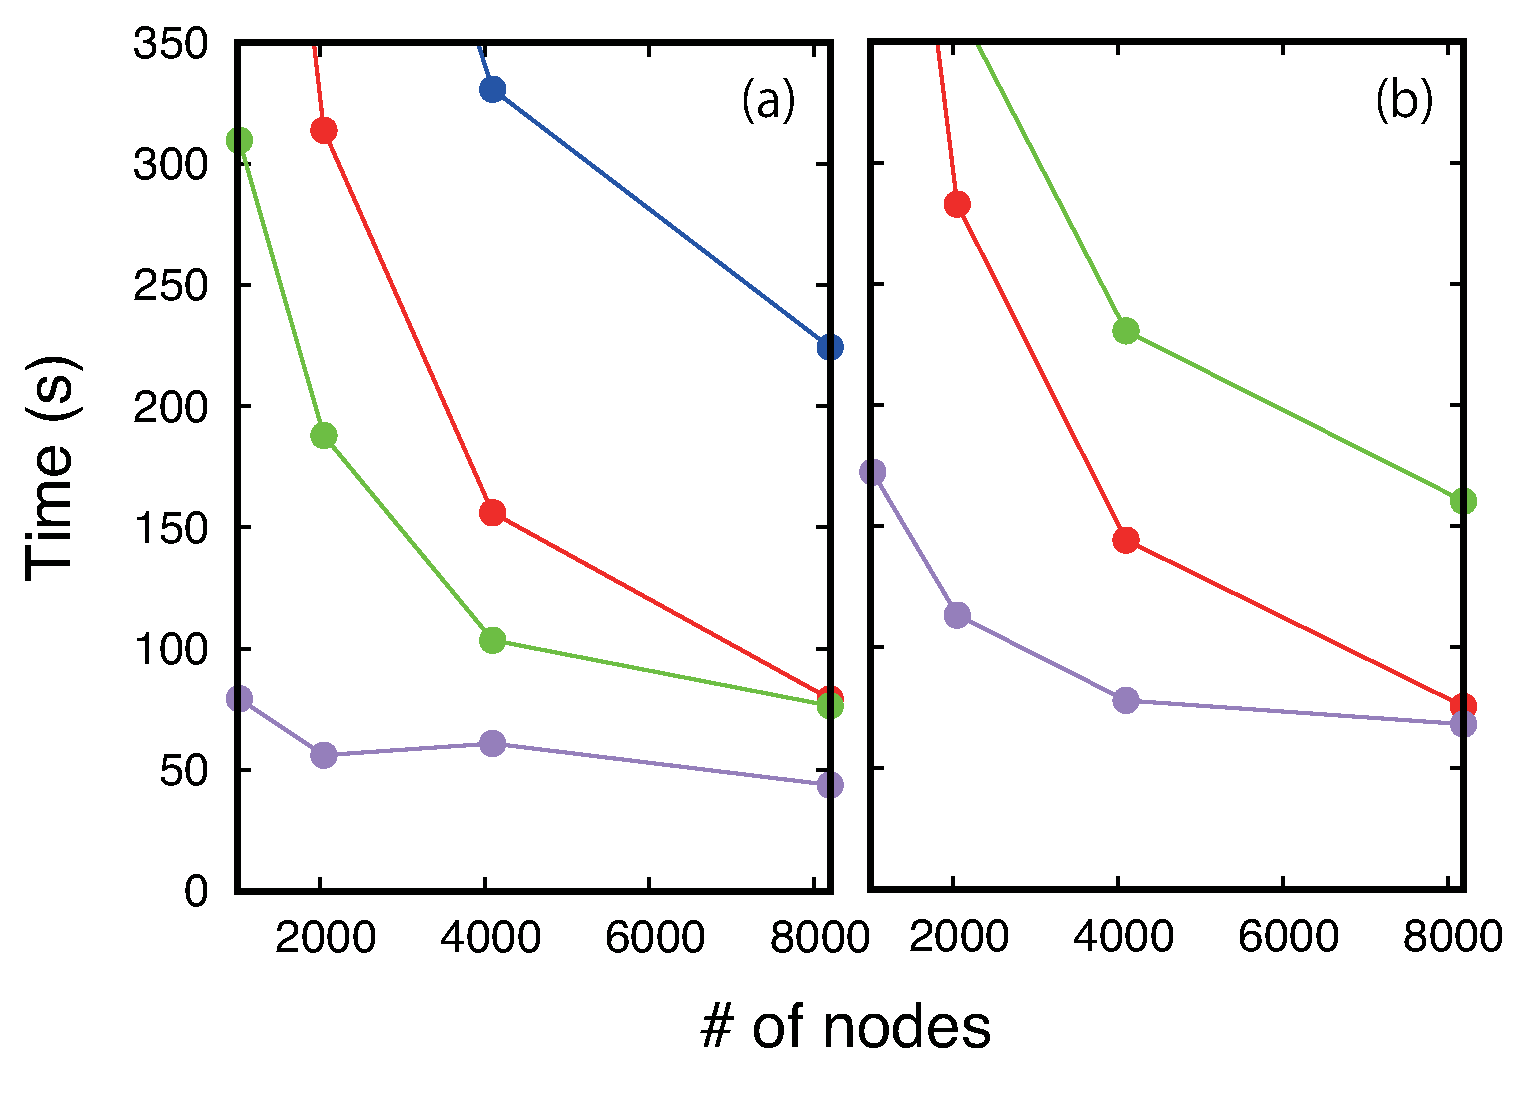
\includegraphics[width=0.525\textwidth]
{research/nakajima/ps_node.eps}
\caption{Computational time of two-electron repulsive integrals in glucose-alanine chain with 8,202 basis functions (a) and H$_2$O molecular cluster with 10,128 basis functions (b) as a function of used nodes.
The red, blue, green, and purple circles denote the analytical, GAPW, PS, and PS-GAP methods, respectively.}
\locallabel{fig:ps_node}
\end{figure}

\subsubsection{Development of massively parallel algorithm of linear response time-dependent density functional theory for excited-state calculations on peta-flops supercomputers}
Linear response time-dependent density functional theory (LR-TDDFT) is an efficient approach for the calculation for excited-states of large molecules.
In the previous study, we developed the MPI/OpenMP hybrid parallel code of LR-TDDFT calculations with random phase approximation (RPA) and Tamm–Dancoff approximation (TDA) [Int. J. Quant. Chem. 115,349 (2015).] in NTChem software.
However, the parallel scalability of this code was limited up to about 1,000 MPI processes on the K computer due to the problems of the parallelization scheme and the I/O overhead of the Davidson diagonalization in the LR-TDDFT calculations.
In this FY, we have developed a new MPI/OpenMP hybrid parallel algorithm for LR-TDDFT/RPA and LR-TDDFT/TDA calculations.
In this algorithm, we have devised an efficient parallelization scheme of the Davidson diagonalization utilizing more than 1,000 MPI processes on the peta-scale supercomputers such as the K computer.
In this scheme, the Davidson diagonalization is parallelized utilizing the distributed memory avoiding the I/O operation reading and writing data to disks.
Vectors needed for Davidson diagonalization (trial vectors, sigma vectors, and residual vectors) are divided to the two-dimensional blocks, and these blocks are distributed to each process.
Matrix-matrix and matrix-vector multiplications evaluating the residual vector and orthogonalization of trial vectors are the computation demanding tasks in the Davidson diagonalization.
These multiplications are performed efficiently applying the OpenMP parallelized basic linear algebra subprograms (BLAS) library.
The scalability of parallel algorithm has been evaluated performing some test calculations of large nano-size molecules.
The largest calculation is the calculation of crambin protein (PDB ID: 1CRN) at the LR-TDDFT/RPA/def2-SVP level (642 atoms 6,177 atomic orbitals (AOs), and 50 excited states) using from 768 to 7,680 nodes of the K computer.
The parallel scalability is good up to 4,608 nodes. Parallel speedups are 80\% and 57\% using 1,536 nodes and 4,608 nodes, respectively. 
The elapsed time is 251 minutes using 4,608 nodes, which demonstrates that the LR-TDDFT excited state calculations of molecular materials and biological molecules contacting up to 600 atoms and 6,000 AOs become routinely possible utilizing the K computer.
The new parallel LR-TDDFT code has been released with NTChem 2013 Version 7.0 on Dec. 2015.

\subsubsection{Development of analytical energy gradient for two-component relativistic time-dependent density functional theory with spin–orbit interaction}
Precise information on excited state potential energy surfaces is the most important prerequisite for a deeper understanding of photochemical reaction or the shape of absorption and luminescence spectra.
In particular, the inclusion of spin–orbit coupling and other relativistic effects is crucial for a proper description of excited-state characters, relaxation dynamics, radiative and nonradiative decay pathways, as well as lifetimes and reactivity for systems containing heavy elements.
The development and efficient implementation of an analytic gradient theory for reliable theoretical models incorporating both electron correlation and relativistic effects has been awaited.
Recently, we have developed two-component relativistic time-dependent density functional theory with spin–orbit interactions (SO-TDDFT), which is becoming popular methodologies for computing excited states containing heavy elements because of its reasonable cost and relatively high accuracy.
In this work, we have implemented the analytical gradient for two-component relativistic TDDFT with spin–orbit interactions in the NTChem program.
Our implementation is based on the derivation of the geometrical derivatives for nonrelativistic TDDFT presented by Furche and Ahlrichs.
The noncollinear exchange-correlation potential presented by Wang {\it et al}. has been applied.
The higher-order matrix elements of the noncollinear exchange-correlation kernel for the relaxed one-particle and two-particle density matrices have been derived and implemented into efficient computer codes with the aid of a newly-developed computerized symbolic algebra system.
In addition, various DFT functionals including the recently proposed range-separated hybrid functionals are applicable to the calculations of excitation energy for spin–orbit coupled states.

\subsubsection{Development of a method for electronic-structure calculations based on self-energy functional theory}
Electronic-structure calculations based on the density functional theory (DFT) have been used in quantum chemistry and providing reliable explanations and predictions of many molecular systems.
While the elaboration of techniques of DFT-based calculations is continued in the community, the limitation of the framework of DFT is known to exist and should be overcome, which is problematic particularly for strongly correlated systems.
For such systems, model Hamiltonians have been used traditionally, in which only few adjustable parameters looking important are often introduced by hand.
Among many approaches proposed so far, the approach based on the self-energy functional theory (SFT) [Potthoff, Eur. Phys. J. B 32 (2003) 429.] is promising.
It has been applied to systems with model Hamiltonians such as a Hubbard chain [Potthoff, Eur. Phys. J. B 36 (2003) 335.] and NiMnSb [Allmaier {\it et al}, Phys. Rev. B 81 (2010) 054422.],
however, no calculation based purely on SFT has not been reported to our knowledge.
Since a SFT-based calculation uses the result of exact diagonalization for the subspace appropriately chosen from the entire Hilbert space, it is expected that the many-body effects are taken into account accurately for describing the strongly correlated system.
We started to develop a method for SFT-based quantum chemistry calculations.
Specifically, we first construct the second-quantized Hamiltonian by calculating one- and two-electron integrals for a molecule and divide the entire Hilbert space into the subspaces
so that as many the molecular orbitals in the vicinity of the Fermi level are contained in one of the subspaces as computationally possible.
We then perform exact diagonalization for the subspaces and calculate the thermodynamic potential of the molecule [Potthoff, Eur. Phys. J. B 32 (2003) 429.] from the self-energies $\Sigma$ of the subspaces as $\Omega = F[\Sigma] - \mathrm{Tr} \ln (-G_0^{-1} + \Sigma)$,
where $F [\Sigma]$ is the universal functional of the self-energies and $G_0$ is the non-interacting Green's function.

\subsubsection{Theoretical study on the cooperative exciton dissociation process based on dimensional and hot charge-transfer state effects in an organic photocell}
In recent years, organic electronics devices such as electroluminescent displays, transistors, and photocells, have actively been studied because of various properties of organic materials, such as lightweight, thin film structures, flexibility, manufacturing costs, design, and so on.
We have been studying organic photocell devices.
It is critical to understand the energy conversion mechanism from the solar photon flux in organic semiconductors, especially the dynamics of strongly bound electron–hole pairs (excitons).
In organic photocells, excitons are first created by absorbing photons.
They then diffuse to the donor–acceptor interface of the organic semiconductor.
Finally, they are dissociated to create free electrons and holes after the electron (charge) transfer process.
Here, we studied the cooperative exciton dissociation process based on dimensional and hot charge transfer state effects.
In last FY, we introduced a local temperature to handle with the hot charge-transfer (CT) sate, and calculated the exciton dissociation probability based on the one-dimensional organic semiconductor model.
Although the hot CT state plays essential roles, the probabilities calculated are not enough high to efficiently separate bounded electron-hole pairs.
In this FY, therefore, we focused on the dimensional effect together with the hot CT state effect.
We showed that cooperative behaviors between both effects can significantly improve the exciton dissociation process.

\subsubsection{Development of trajectory surface hopping algorithm for the time- dependent density functional theory: Toward the understanding of working mechanisms of organic photovoltaic solar cells}
The solar cell can convert solar energy into electric energy and is a valuable resource of clean energy that is free from environment pollution.
While people have used silicon-based solar cells widely in a real life, organic photovoltaic devices are considered to be promising in a next generation due to their versatility, easy processing, low cost, and so on.
The photo-energy conversion efficiency is a critical factor in the development of new solar cells.
So it is necessary to derive a valuable relationship between the conversion efficiency and the properties of constituent organic molecules.
Nowadays, quantum chemistry calculations routinely afford (1) the energy gap between the highest occupied molecular orbital and lowest unoccupied molecular orbital, (2) excitation energies, and (3) oscillator strengths.
Although these data give guidelines to develop new photo-functional materials, they are insufficient to reveal the details of photochemical processes after light absorption;
how solar cells work relies on the mechanisms of the exciton (electron-hole pair) generation and its separation/migration.
Therefore, it is desirable to simulate the relaxation processes on the excited-state potential energy surfaces (PESs) directly and to observe the real-time behavior of electron–hole pair.
A large size of organic dye molecules hampers the on-the-fly molecular dynamics simulation by sophisticated wavefunction approaches.
Furthermore, photochemical processes involve a large number of PESs, and one must take accounts of non-adiabatic transition between these electronic states.
To satisfy these requirements, we have implemented a combined method of time-dependent density functional theory (TD-DFT) and trajectory surface hopping (TSH) algorithm.
For now, the TSH input data was taken from the TDDFT output given by the program package GAMESS.
The TSH program needs the non-adiabatic coupling vector (NACV), which is not trivial at the TDDFT level of theory.
Instead of deriving analytic NACV, we introduced isotropic scalar NAC as the overlap of wavefunctions at consecutive time steps and computed it on the fly.
Some test calculations in progress show the efficiency and robustness of the proposed method.

\subsection{Applications of original molecular theory to new materials and drugs}
\subsubsection{Theoretical study on spin-forbidden transitions of metal complexes by two-component relativistic time-dependent density functional theory}
Spin-forbidden transitions of metal polypyridyl sensitizers are studied by the two-component relativistic time-dependent density functional theory with spin–orbit interaction based on Tamm–Dancoff approximation.
The spin-forbidden transitions for a phosphine-coordinated Ru(II), DX1, as well as the modified DX1 complexes whose Ru is replaced with Fe and Os, are calculated.
The role of the central metals in spin-forbidden transitions is discussed toward the exploration for new efficient sensitizers.
In addition, we study spin-forbidden transitions of Os polypyridyl sensitizers.
The absorption spectra, including spin-forbidden-transition peaks, for the Os complexes are reasonably reproduced in comparison with the experimental ones.
The extension of the conjugated lengths in the Os complexes is investigated and found to be effective to enhance photo absorption for spin-allowed transitions as well as spin-forbidden ones.
This study provides fruitful information for a design of new dyes in terms of conjugation lengths.

\subsubsection{Large-Scale QM/MM calculations of hydrogen bonding networks for proton transfer and water inlet channels for water oxidation - Theoretical system models of the oxygen-evolving complex of photosystem II}
In order to confirm theoretical system models of photosystem II (PSII), quantum mechanics (QM)/ molecular mechanics (MM) calculations using a large-scale QM model (QM Model V) have been performed to elucidate hydrogen bonding networks and proton wires for proton release pathways (PRPs) of water oxidation reaction in the oxygen-evolving complex (OEC) of PSII.
Full geometry optimizations of PRP by the QM/MM model have been carried out starting from the geometry of heavy atoms determined by the recent high-resolution X-ray diffraction (XRD) experiment on PSII refined to 1.9 \AA\ resolution.
The optimized MnMn and CaMn distances by large-scale QM/MM are consistent with the EXAFS results, removing out the discrepancy between the refined XRD and EXAFS.
Computational results from QM/MM calculations have demonstrated the labile nature of the MnaO(5)Mnd bond of the CaMn4O5 cluster in the OEC of PSII which allows left (L)-opened, quasi-central (CQ)-, and right (R)-opened structures.
This confirms the feasibility of the left- and right-hand scenarios for water oxidation in the OEC of PSII that are dependent on the hydrogen bonding networks.
The QM/MM computations have elucidated the networks structures: hydrogen bonding O. . .O(N) and O. . .H distances and O(N)H. . .O angles in PRP, together with the ClO(N) and Cl. . .H distances and O(N)H. . .Cl angles for chloride anions.
The obtained hydrogen bonding networks are fully consistent with the results from XRD and available experiments such as EXAFS, showing the reliability of our theoretical system model that is crucial for investigations of functions of PSII such as water oxidation.
The QM/MM computations have elucidated possible roles of chloride anions in OEC of PSII for proton transfers.
The QM/MM computational results have provided useful information for the understanding and explanation of several experimental results obtained with mutants of the OEC of PSII.
The possible implications of the present results are discussed in relation to our theoretical system models of PSII, strong or weak perturbations of the system structures by mutations, damage-free X-ray free-electron laser structure of PSII, and bioinspired working hypotheses for the development of artificial water oxidation systems which use 3d transition metal complexes.

\subsubsection{Full geometry optimizations of the CaMn$_4$O$_4$ model cluster for the oxygen evolving complex of photosystem II}
Full geometry optimizations of ([CaMn$_4$O$_4$(CH$_3$COO)$_8$(py)(CH$_3$COOH)$_2$], (py: pyridine) (1)) were performed at the UB3LYP theoretical level.
This model 1 is a theoretical model for the synthetic model ([CaMn$_4$O$_4$(ButCOO)$_8$(py)(ButCOOH)$_2$], (But: t-butyl) (2)) which closely mimics the native oxygen evolving complex (OEC) in photosystem II.
It was shown that the X-ray structure of 2 was well reproduced by 1 in the (Mn1(III), Mn2(IV), Mn3(IV), Mn4(III)) valence state with the unprotonated O5 (O5 = O2-), and two different valence states were obtained in the one-electron oxidized state.
Importance of the Jahn-Teller effect of the Mn(III) site for the structural deformations was presented.

\subsubsection{Theoretical study on selective recognition of biomolecule in supramolecule}
The purpose of this study is to analyze and understand of molecular recognition using quantum chemical calculations.
In 2009, Sawada {\it et al}. observed only single nucleotide duplex could form stably in water inside artificial cage-like supramolecule [Sawada {\it et al}. Nature Chemistry 1, 53 (2009).].
Since it was said that at least four complementary nucleotide base pairs had been necessary in order to form stable structure in water, this result can be called great progress.
In our study, we approached this issue in terms of the molecular orbital (MO) method and tried to clarify structural stability and selectivity mechanism of the target.
The selectivity in this target is that single base pair is spontaneously formed as anti-Hoogsteen (AH) type, not Watson–Click (WC) type.
In order to elucidate this selectivity, we prepared both AH-type and WC-type nucleotide duplex and performed structure optimizations with/without surrounding cage-like supramolecule.
According to the result, AH-type structure is more stable than WC-type one by 53.1 kcal/mol inside cage-like supramolecule and the same energy gain becomes only 0.2 kcal/mol without the supramolecule.
Moreover, our calculation indicates the importance of non-covalent bonding between the cage and nucleotide duplex which originates from $\pi$-$\pi$/CH-$\pi$ interaction.

\section{Schedule and Future Plan}
In the next financial year, we will continue to develop new algorithms and improve the parallel efficiency of the NTChem2013 suit of program.
In the present implementation of LR-TDDFT, the replicated memory algorithm is adopted for the evaluations of Fock like matrix.
This situation limits the application of the present code to the systems having less than 7,000 AOs on the K computer.
To overcome this problem, we are developing the distributed-memory parallel code of Fock-like matrix calculations.
Furthermore, the spin–orbit coupling often plays an important role for the excites states containing heavy elements.
We are developing the massively parallel algorithm and code of two-component relativistic LR-TDDFT to account for the spin–orbit interactions explicitly in the excited state calculations.
We will also develop transition properties and nonadiabatic coupling constant matrix elements, which are the key quantity in the description of excited-state dynamics.
In addition, for further acceleration of the PS and PS-GAP methods, we are planning to do coding and tuning of related programs in NTChem so that we will apply the improved PS and PS-GAP methods to several large molecular systems.
For self-energy functional theory (SFT), we further will continue to parallelize the calculations of one- and two-electron integrals and of exact diagonalization and of Green's functions.
The implementation of SFT-based electronic-structure calculations for periodic systems are in progress.
It is interesting to develop a unified approach to the understanding of the internal conversion (IC) and intersystem crossing (ISC) processes.
The suppression of unfavorable quenching pathways may help the design of new organic materials with high efficiencies.
One of the attractive points in NTChem program is the availability of relativistic methods.
The spin–orbit TDDFT (SO-TDDFT), in particular, can deal with both singlet and triplet states on an equal footing.
The SO-TDDFT/TSH simulation involving both spin states can be performed in a similar way as the singlet-state-only TSH because a natural extension of the conventional TDDFT coupling yields the SO-TDDFT counterpart.
Another direction is to develop a hybrid method of quantum mechanics/molecular mechanics (QM/MM).
Bulk heterojunction solar cell, for example, is a composite system of p- and n-type layers.
It is natural to split the whole system to reduce the computational cost.
The QM method is applied to the small region, the interface between the p- and n-type materials, while the remaining part is treated as MM.
The method will give insights into the environmental effects on charge transport dynamics that occurs at the interface.
We earnestly hope that NTChem will be an important tool leading the way toward a new frontier of computational molecular science.


%%% DO NOT EDIT BELOW

\section{Publications}

%\printbibliography[keyword=journal, heading=subbibliography, title={Journal Articles}, prefixnumbers={1-}, resetnumbers=true]
%\printbibliography[keyword=proceedings, heading=subbibliography, title={Conference Papers}, prefixnumbers={2-}, resetnumbers=true]
%\printbibliography[keyword=invited, heading=subbibliography, title={Invited Talks}, prefixnumbers={3-}, resetnumbers=true]
%\printbibliography[keyword=poster, heading=subbibliography, title={Posters and Presentations}, prefixnumbers={4-}, resetnumbers=true]
%\printbibliography[keyword=deliverable, heading=subbibliography, title={Patents and Deliverables}, prefixnumbers={5-}, resetnumbers=true]

\printbibliography[keyword=journal, heading=subbibliography, title={Journal Articles}, resetnumbers=true]
\printbibliography[keyword=proceedings, heading=subbibliography, title={Conference Papers}]
\printbibliography[keyword=invited, heading=subbibliography, title={Invited Talks}]
\printbibliography[keyword=poster, heading=subbibliography, title={Posters and Presentations}]
\printbibliography[keyword=deliverable, heading=subbibliography, title={Patents and Deliverables}]

\end{refsection}
